% Created 2025-02-27 Thu 18:35
% Intended LaTeX compiler: pdflatex
\documentclass[11pt]{article}
\usepackage[utf8]{inputenc}
\usepackage[T1]{fontenc}
\usepackage{graphicx}
\usepackage{longtable}
\usepackage{wrapfig}
\usepackage{rotating}
\usepackage[normalem]{ulem}
\usepackage{amsmath}
\usepackage{amssymb}
\usepackage{capt-of}
\usepackage{hyperref}
\usepackage{minted}
\author{Ross Mikulskis}
\date{\today}
\title{RT-USB Streaming Protocol}
\hypersetup{
 pdfauthor={Ross Mikulskis},
 pdftitle={RT-USB Streaming Protocol},
 pdfkeywords={},
 pdfsubject={},
 pdfcreator={Emacs 29.4 (Org mode 9.8-pre)}, 
 pdflang={English}}
\begin{document}

\maketitle
\tableofcontents

\section{Problem statement}
\label{sec:org0919e67}
\subsection{Problem definition}
\label{sec:orgc28f8f3}
Safety-critical systems and manufacturing workloads in factories require
timing and predictability guarantees for proper execution. For example, an
autonomous car reading lidar sensor data requires end-to-end latency guarantees
within a margin to be able to stop when detecting a pedestrian. Similarly, in
precision manufacturing pipelines of microprocessors, robots need to be
synchronized to a high degree degree of accuracy to ensure no anamolies in
coordinated execution.

Currently, ROS2 (Robot Operating System 2) is the de-facto pub-sub framework for
robotics systems. The issue with ROS2 is that there may be hardware interrupts
that disrupt proper execution flow, so end-to-end latency guarantees are
weak.

The problem is that there is no data distribution service (DDS) that provides
real-time guarantees.
\subsection{Problem importance}
\label{sec:org5764cb9}
We need a real-time DDS for safety critical systems to ensure predictability
guarantees in workload executions. The aformentioned examples of factories and
autonomous vehicles are clear demonstrations of this need; however, a real-time
DDS also has many applications in optimizing workloads in e.g. high frequency
stock trading, or cluster coordinated execution. Scheduling work on nodes with
time as a first-class resource enables power efficiency and deterministic CPU
utilization (c.f. Rate-Monotonic Scheduling). Therefore, a real-time DDS that
scales across nodes may lay the groundwork for building a scalable,
highly-efficient supercomputer.
\subsection{Who benefits from solving this?}
\label{sec:orge2b0673}
\section{Proposed solution}
\label{sec:org1299f81}
In the Quest Lab we have been developing RT-DDS, a real-time pub-sub data
distribution service, which provides strong end-to-end latency and throughput
guarantees through exploiting the Quest VCPU (Virtucal CPU) construct that
ensures timing and predictability in task execution. Upon an interrupt, Quest
spawns an IO VCPU with equal priority to the Main VCPU that was preempted, and
handles the bottom-half of the interrupt in parallel to allow for near-seamless
execution of the Main VCPU's task.

We propose RT-DDS across hosts as the first real-time DDS to span hosts and
provide coordinated execution with end-to-end latency requirements. We will
use USB links to connect nodes and communicate host-to-host using the
USB extensible debug cabability (xDbC), first on Linux, then on Quest to provide
stronger timing and predictability guarantees than ROS2. Using xDbC we will need
to construct a real-time USB protocol which incorporates acknowledgements for
replicating the state of the endpoint buffers on each host as well as provide
a scheduling mechanism at the OS USB driver level for rate-matched transfers.

\begin{figure}[htbp]
\centering
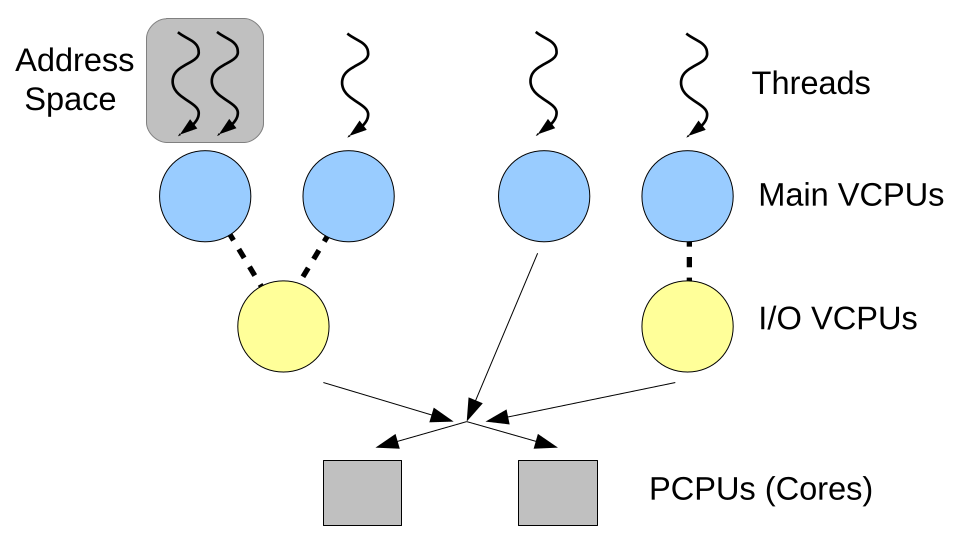
\includegraphics[width=.9\linewidth]{./vcpu_hierarchy.png}
\caption{\label{fig:org4b4b047}From boomerang paper; processes which contain thread(s) bound to a VCPU (Main), which is bound to a PCPU (core). Each Main VCPU may have a corresponding IO VCPU with the same budget C and period T to handle the bottom-half of interrupts.}
\end{figure}    

We can guarantee end-to-end latency requirements because of the Quest VCPU
construct because Quest schedules processes with RMS (Rate Monotonic Scheduling)
using the Liu \& Layland upper bound, which guarantees that a feasible schedule
that will always meet deadlines exists if the CPU utilization is below a specific
bound. Additionally, the bottom half of interrupts are handled by IO VCPUs
so Main VCPUs can execute with negligible performance impact upon an interrupt.

With these timing and predictability guarantees at the operating system level,
given an end-to-end latency \(e\), RT-DDS binds each task in the pipeline to a
VCPU of period \(T=\frac{e}{num\_pipeline\_stages}\) to rate match all services
in the pipeline (they produce 1 unit of work, reading from all inputs, processing
the inputs, and writing to all outputs, at the same rate)
oand \(C=max\_execution\_time(f)\)
where \(f\) is the service's function and a pipeline stage is a stage in the
pipeline where the services in it can execute in parallel (i.e. they have all the
data they need). c.f. topological sort, see \ref{fig:org6461418} where the 4 pipeline stages are
vertically aligned; services \(B\) and \(C\) are in the same stage.
\section{Expectations}
\label{sec:org9798293}
\subsection{Pub-sub with end-to-end and throughput latency guarantees}
\label{sec:orgf82a1f2}
Currently RT-DDS is limited to a single host, with
data streaming across shared memory communication; however, enabling RT-DDS to
span across hosts on Linux will situate it as a mainstream alternative DDS to
ROS2. Upon completion of this project, strong real-time guarantees will become
available for cluster-level coordinated execution for the first time.
\section{Experimental plan}
\label{sec:org1467aa6}
Linux does not provide the same timing guarantees as Quest; however, for fair
comparison we will first compare RT-DDS on Linux against ROS2 on Linux. Then
we will do a comparison of RT-DDS on Quest against ROS2 on Linux to demonstrate
the strength of running the DDS on a real-time OS.
\subsection{Datasets}
\label{sec:orga168572}
All of our data will be audio data, which on which we will apply digital
signal processing (DSP) functions from the soundpipe library. 
\subsection{Experiments}
\label{sec:org5d35b43}
All experiments will aim to minimize the end-to-end latency, so hopefully
on the order of magnitude of 100s of microseconds per audio sample batch.
44khz is 25 microseconds per sample, but if we cannot achieve that, then
we can batch samples at a lower frequency.
\begin{enumerate}
\item 1khz sine wave (unsigned 16 bit), 2 services:
\begin{enumerate}
\item Pub1 (Host 1): read and stream \texttt{1khz\_sine.raw}
\item Sub1 (Host 2): read from Pub1 over USB and flush to a Teensy 4.1 board
connected to an audio sink to play the audio data
\end{enumerate}
\item complex DAG with synchronized merging of audio (from 1):
$$A|B,C|D|E$$ where | is a subscription, and B|C,D|E means C and D subscribes to
B and E subscribes to C and D (See the figure below)
\end{enumerate}

\begin{figure}[htbp]
\centering
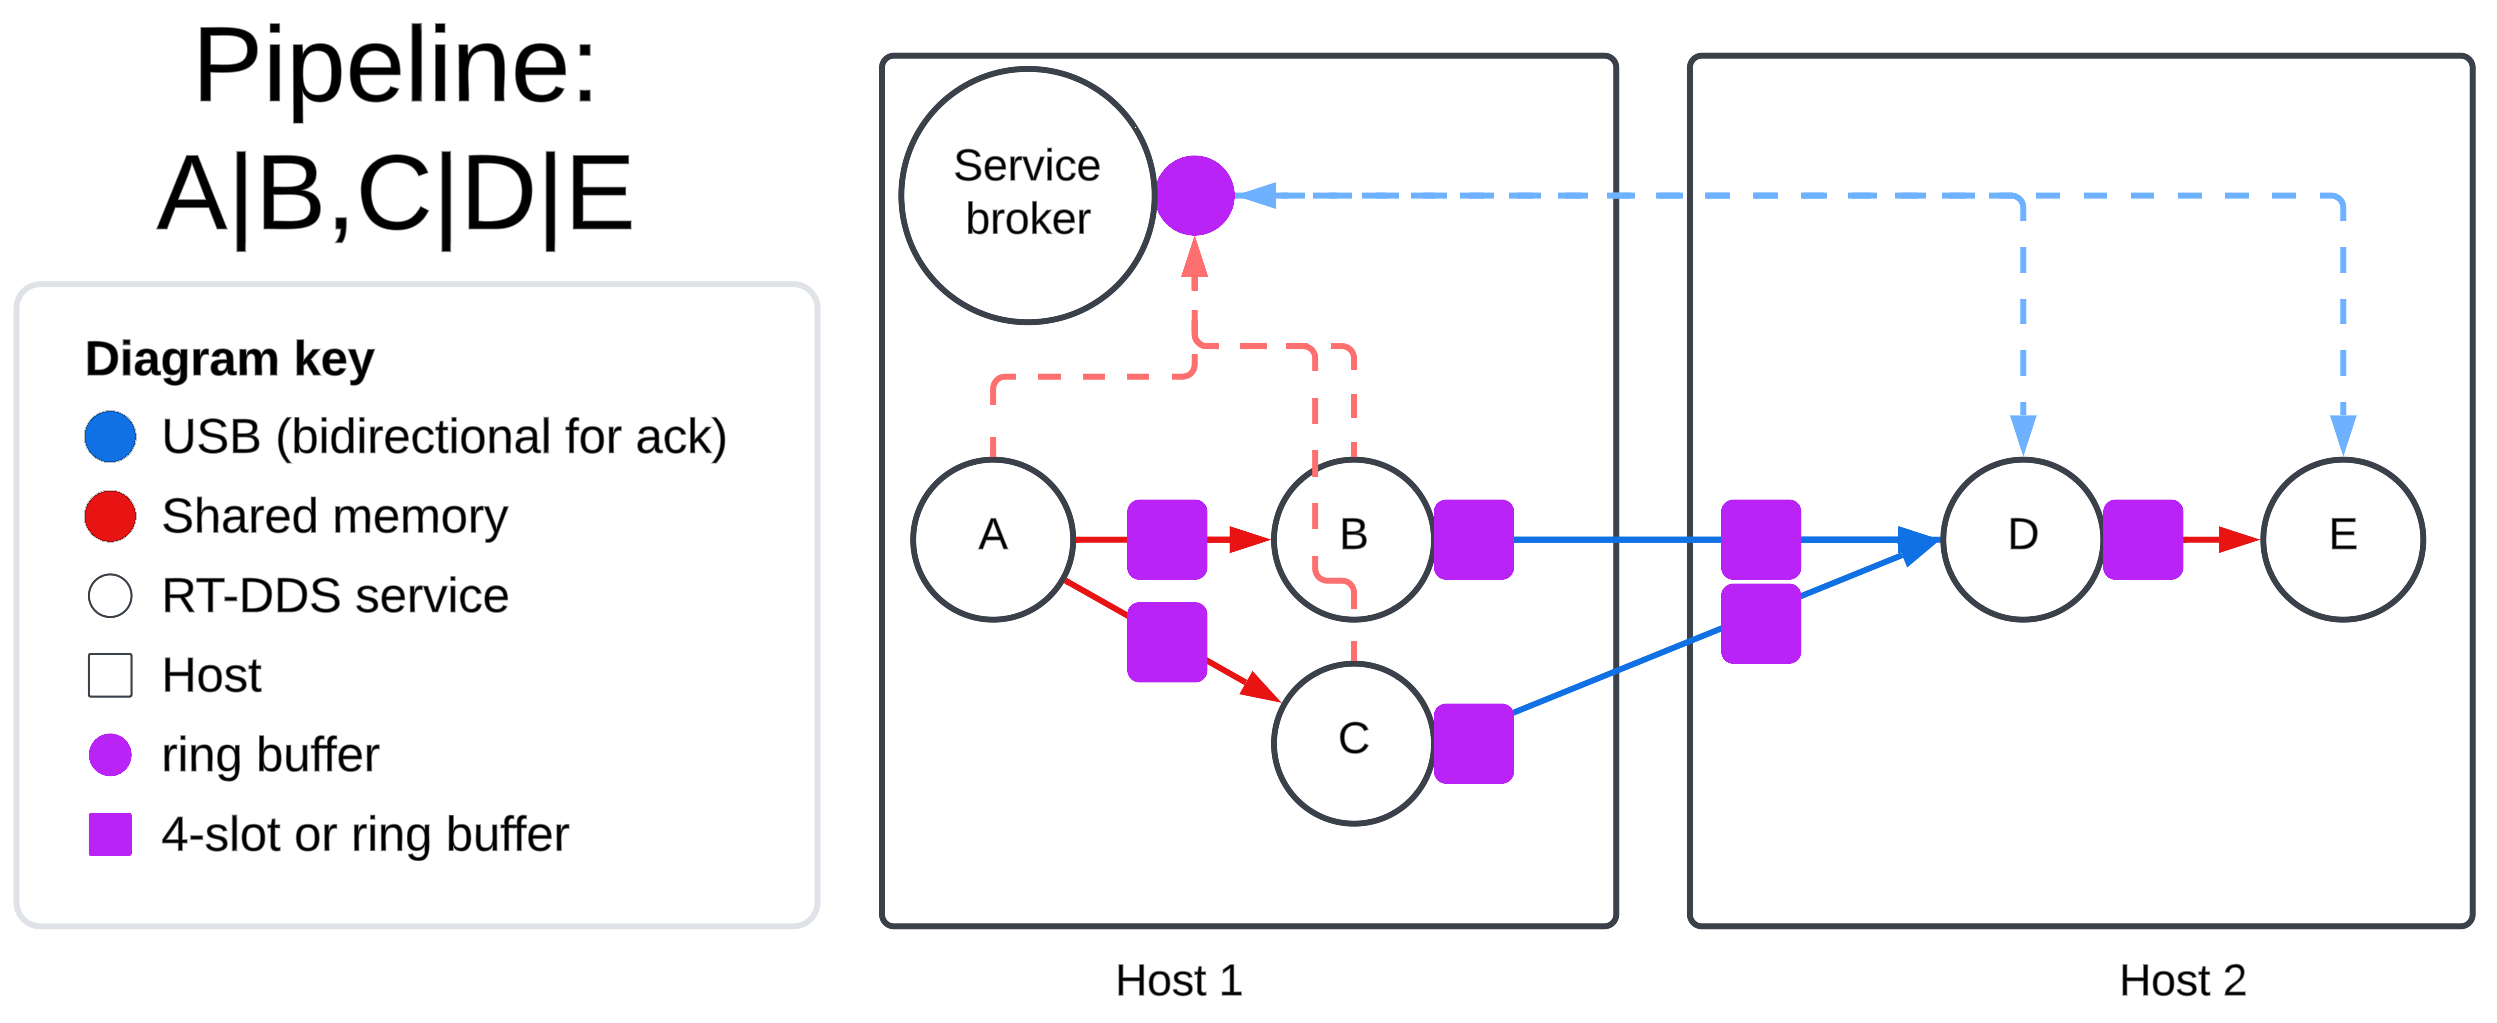
\includegraphics[width=.9\linewidth]{./pipeline.png}
\caption{\label{fig:org6461418}Diagram of \(A|B,C|D|E\). Bidirectional communication over xDbC for acks on buffer state. (Simpson's) 4-slot buffers are for asynchronous communication and ring buffers for synchronous.}
\end{figure}
\subsection{Deploy environment}
\label{sec:org71847aa}
We will be running experiments on 64-bit Ubuntu Linux standalone for ROS2 and
32-bit Yocto Linux as a guest on the Quest-V hypervisor, or possibly standalone
Linux if time allows, for RT-DDS. For a Quest RT-DDS workload, we will do this
on both Quest standalone, and Quest as a Quest-V guest to demonstrate minimal
overhead.
\subsection{How confirm hypothesis}
\label{sec:orgbf4534d}
\begin{enumerate}
\item Measure end-to-end latency and throughput of DDS during both normal
execution and under background process interrupts, e.g. heavy I/O reading
other files in tasks outside of the pipeline.
\item Spectrum analyzer for teensy audio sink to see that the 1khz sine is
preserved and pure.
\item Audio sample sounds good to the ear, we may use a pop song to demonstrate
the synchronization of the split and merge in experiment 2.
\end{enumerate}
\subsection{Equipment}
\label{sec:orgaca0795}
\begin{itemize}
\item 2 DX1100 32-bit hosts
\item USB link
\item Teensy microcontroller
\item audio sink
\item spectrum analyzer (currently have an oscilloscope, need to ask to borrow
from Professor Mancuso possibly)
\end{itemize}
\section{Success indicators}
\label{sec:org6c55355}
\subsection{Outcome of work}
\label{sec:org7a895ff}
RT-DDS works across hosts over USB xDbC. First implemented real-time
DDS available.
\section{Task assignment/milestones}
\label{sec:org1ecf03a}
\subsection{{[}2/23, 3/02)}
\label{sec:org726e2fa}
\begin{itemize}
\item RT-DDS working on Linux over Quest-V, single host
\item draft of USB RT-packet streaming protocol
\end{itemize}
\subsection{{[}3/02, 3/09)}
\label{sec:org1574ca0}
\begin{itemize}
\item begin implementation of USB RT-packet streaming protocol
\end{itemize}
\subsection{{[}3/07, 3/14)}
\label{sec:org443015a}
\begin{itemize}
\item finish implementation of USB RT-packet streaming protocol
\end{itemize}
\subsection{{[}3/14, 3/20)}
\label{sec:org225c21a}
\begin{itemize}
\item implement both experiments for RT-DDS
\end{itemize}
\subsection{3/20: Midterm presentation due}
\label{sec:orgb416e18}
\subsection{{[}3/21, 3/28)}
\label{sec:orgb09d686}
\begin{itemize}
\item implement both experiments on ROS2
\end{itemize}
\subsection{{[}3/28, 4/04)}
\label{sec:orgf0f0cb8}
\begin{itemize}
\item Spectrum analyzer analysis and timing analysis of experiments
\end{itemize}
\subsection{{[}4/04, 4/11)}
\label{sec:org2532d0b}
\begin{itemize}
\item RT-DDS on Linux standalone
\end{itemize}
\subsection{{[}4/11, 4/18)}
\label{sec:org49d7c92}
\begin{itemize}
\item Write up presentation
\end{itemize}
\subsection{{[}4/18, 4/22)}
\label{sec:org688a064}
\begin{itemize}
\item Finish any unfinished tasks
\end{itemize}
\subsection{4/23: Final presentation due}
\label{sec:org5f83f0b}
\section{Relevant papers}
\label{sec:org2727af5}
\begin{enumerate}
\item A. Eisenklam, W. Hedgecock and B. C. Ward, ``Job-Level Batching for Software-Defined Radio on Multi-Core,'' in 2024 IEEE Real-Time Systems Symposium (RTSS), York, United Kingdom, 2024, pp. 375-387, doi: 10.1109/RTSS62706.2024.00039.
\end{enumerate}
\end{document}
